\section{Results}\locallabel{sec:results}
While our initial motivation for this study was to look at the effect of the
feedback delay on student submission behavior, the data we collected also
allows us to offer new insights into questions previously investigated by other
researchers. The analysis of our submission data lends support to some existing
answers to these questions, and contradicts others. In particular, we compare
our results to those of \spacco{} collected in Spring
2006.~\cite{Spacco:2013:TIP:2462476.2465594}. Where our results differ, we draw
new conclusions using information from both our results, and theirs.

In this section we present the results obtained from an analysis of the 20,777
submissions collected from seven UCSB computer science classes from Winter
Quarter 2013 through Spring Quarter 2014. We seek to answer the following
questions:

\begin{itemize}
\item Section~\localref{sec:early}: Does Starting Early Help?
\item Section~\localref{sec:time}: Does Time Pressure Affect Behavior?
\item Section~\localref{sec:efficiency}: Does Time Pressure Affect Efficiency?
\item Section~\localref{sec:deadline}: Why Do Students Submit Well After an
  Assignment's Deadline?
\item Section~\localref{sec:sub_impact}: Does Delaying Feedback Impact Student
  Submission Behavior?
\item Section~\localref{sec:session}: Does Delaying Feedback Impact Student
  Work Sessions?
\end{itemize}

\subsection{Does Starting Early Help?}
\locallabel{sec:early}

\begin{figure}[!t]
\centering
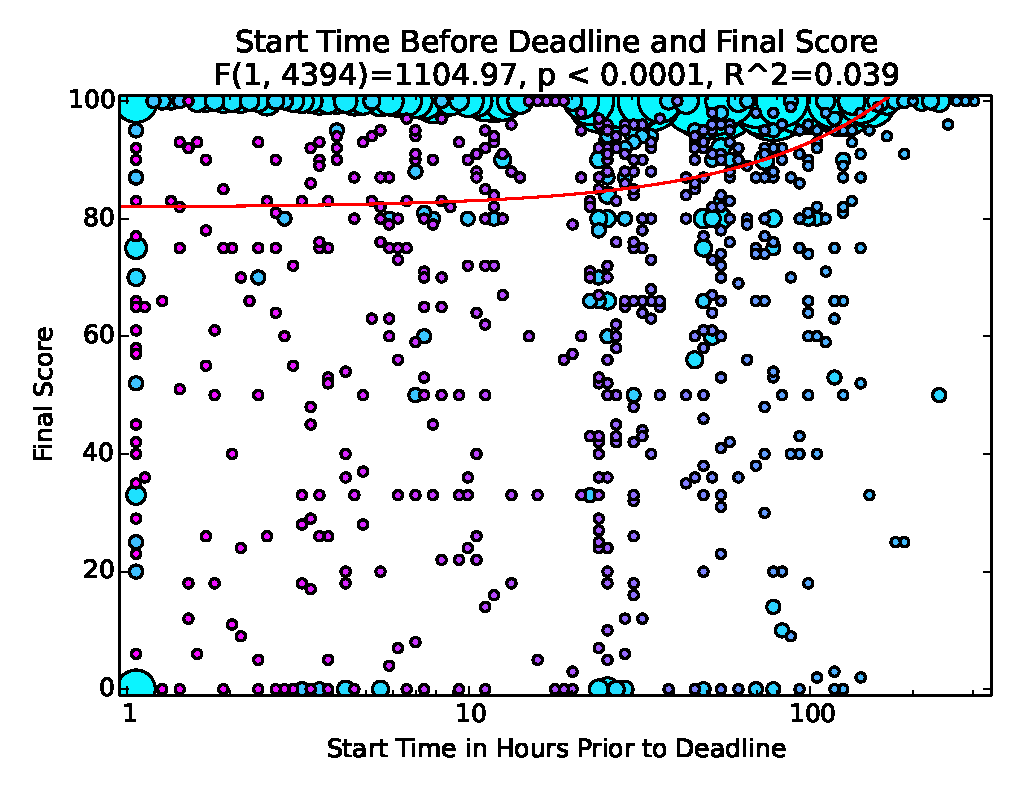
\includegraphics[width=3.3in]{graphs/Start_Time_Before_Deadline_and_Final_Score.eps}
\caption{Compares the number of hours prior to assignment deadline that groups
  started the assignment to the final score they received. Both the size and
  color of each circle correspond to the number of groups represented at that
  position. The circles are plotted such that smaller circles are strictly in
  front of larger circles.}
\locallabel{fig:relative_start_time}
\end{figure}

\begin{figure}[!t]
\centering
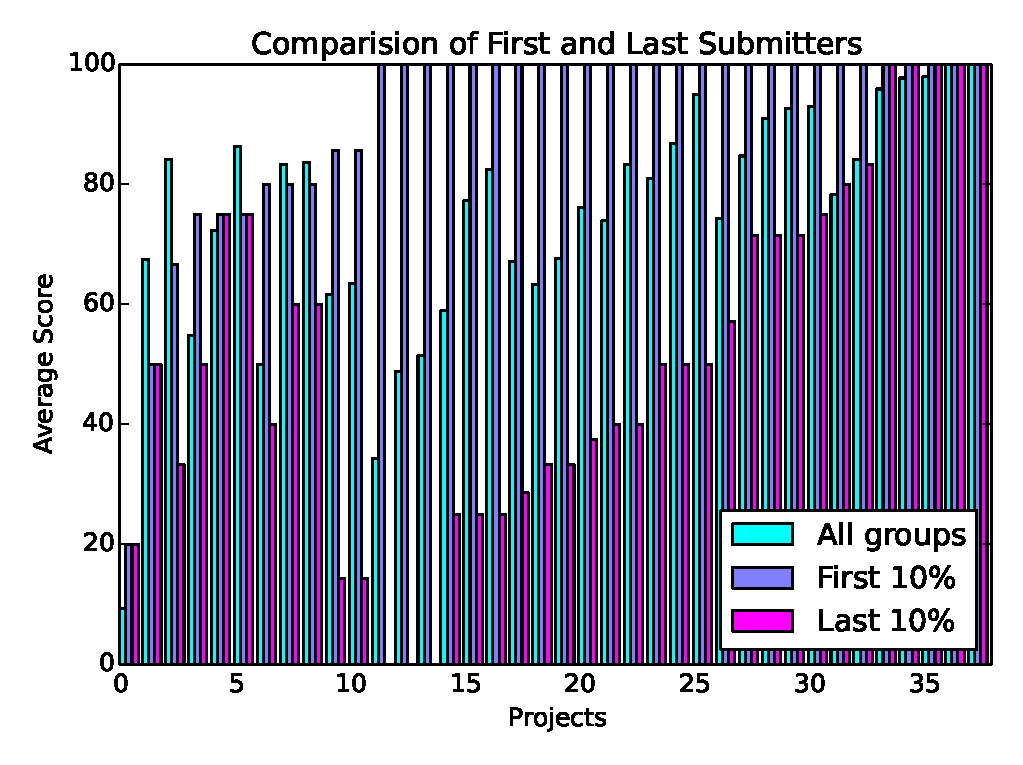
\includegraphics[width=3.3in]{graphs/Comparision_of_First_and_Last_Submitters.eps}
\caption{Compares the average final score of the first 10\% of groups to submit
  to the average and to the last 10\% of groups to submit by assignment. The
  first 10\% of groups to submit had perfect scores on twenty-seven of the
  thirty-eight assignments.}
\locallabel{fig:percent_score}
\end{figure}

Many educators encourage their students to start early on
assignments. Intuitively, starting early gives students more time to receive
feedback from the instructor and teaching assistants in order to make
improvements to the work they submit by the deadline. However, with traditional
assessment, is it unlikely for an instructor to offer multiple early assessment
iterations to all students. With a real-time feedback and assessment system, on
the other hand, starting early additionally offers all students multiple
opportunities for assignment feedback and assessment. Furthermore, the feedback
provided by these systems can then be leveraged by the student and instructor
in office hours.

Prior work in the field has shown that a positive correlation does in fact
exist between starting early and assignment
score~\cite{Spacco:2013:TIP:2462476.2465594,
  Edwards:2009:CEI:1584322.1584325}. We sought to verify that our results are
consistent with those of the prior work.

Figure~\localref{fig:relative_start_time} plots the number of hours before an
assignment is due of a group's first submission against the final score the
group receives. Our data statistically significantly correlate earlier
assignment start times with higher scores. While it may seem odd that groups
can receive 100\% on an assignment having started only an hour or less prior to
the deadline, this result is merely an artifact of our active data
collection. Our data collection methodology only provides a lower bound to how
long prior to assignment deadline a group began working. We verified that a
small number of groups, distributed uniformly across assignments, would make
their first submission in the last hour. This behavior indicates that some
groups mostly worked without using the system in order to receive feedback.

While Figure~\localref{fig:relative_start_time} shows a correlation with start
time and final score, we can break down relative start times even further to a
per-assignment basis. Figure~\localref{fig:percent_score} compares the average
score of the first 10\% of groups to make a submission on an assignment, to
that of all groups, and to the last 10\% of groups to make their first
submission. The assignments are sorted according to the first 10\% value, and
then the last 10\% value. Assignments with fewer than thirty groups are
excluded so that at least three groups make up each of the 10\% categories. Of
the thirty-seven assignments that meet the criteria, the first 10\% of groups
all received 100\% in twenty-six (70\%) assignments, only five (20\%) of which,
where the last 10\% of groups also all received 100\%. In the other twenty-one,
the last 10\% scored significantly worse than the average.

In the cases where the first 10\% of groups did not receive 100\%, there are a
few outliers where the average is higher than the first 10\% of groups to
submit. All of those five cases were lab assignments where each student
attended one of many lab sessions. It is likely that a subset of the first 10\%
groups to submit all emanate from an early lab session where they were directed
to make their first submission at a point they would not otherwise have made
it.

\subsection{Does Time Pressure Affect Behavior?}
\locallabel{sec:time}

\begin{figure}[!t]
\centering
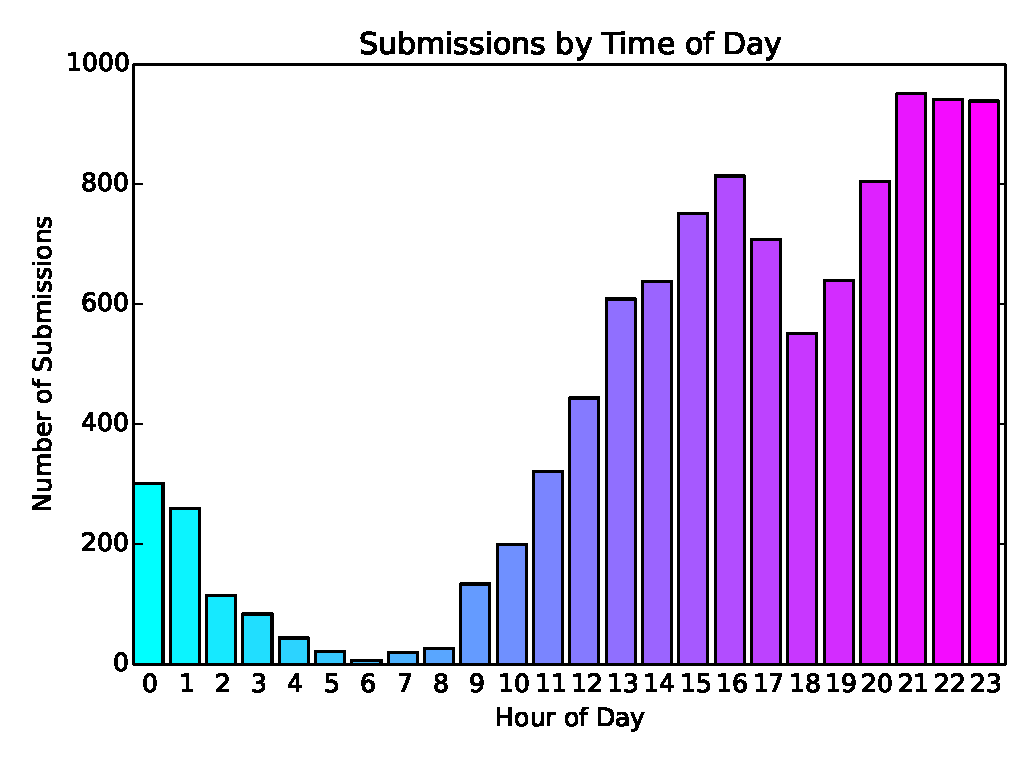
\includegraphics[width=3.3in]{graphs/Submissions_by_Time_of_Day.eps}
\caption{Visualizes the time of day submissions were made excluding submissions
  within a day of their deadline. Note the \PM{4} peak and the larger peak
  starting at \PM{9} lasting through midnight.}
\locallabel{fig:by_time_far}
\end{figure}

\begin{figure}[!t]
\centering
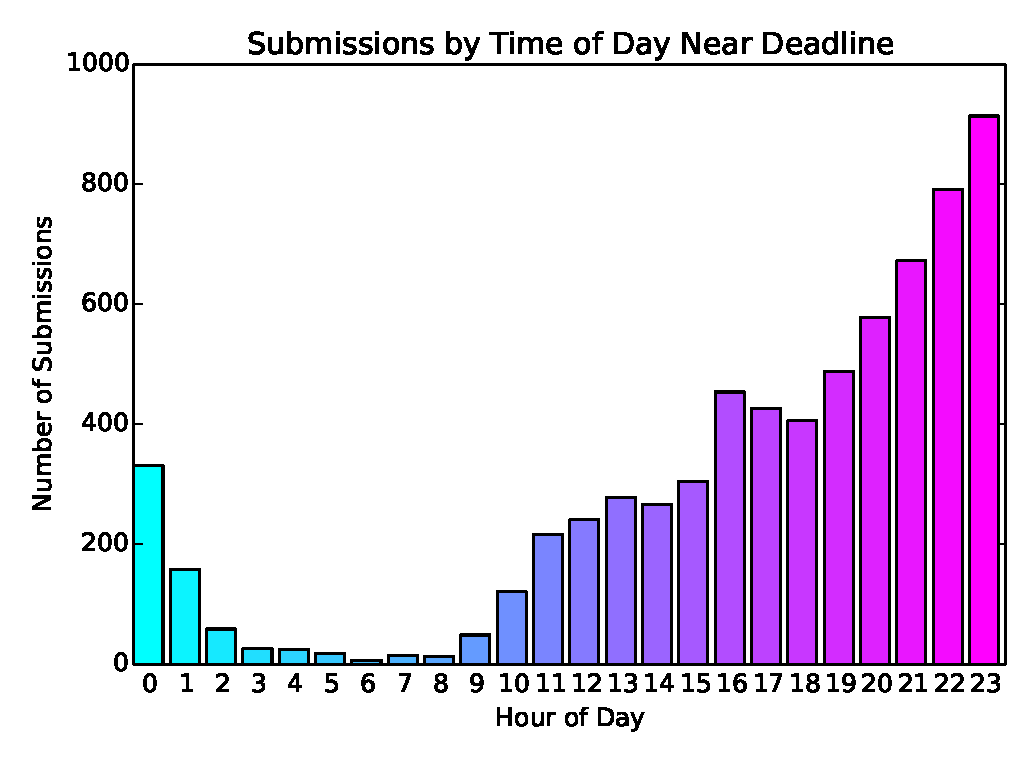
\includegraphics[width=3.3in]{graphs/Submissions_by_Time_of_Day_Near_Deadline.eps}
\caption{Visualizes the time of day submissions were made including only
  submissions within a day of their deadline. The \PM{11} peak corresponds to
  the hour prior to the deadline for most assignments.}
\locallabel{fig:by_time_near}
\end{figure}

Motivated by the work of \spacco{}, we wanted to see if our real-time feedback
and assessment system, which required students to actively make assignment
submissions, measured similar student working behavior. \spacco{} discovered
their students produced the most work in days prior to the deadline at
\PM{4}. The amount of work significantly dropped at \PM{6} and remained nearly
consistent until \AM{1}. Although all of their assignment deadlines were at
\PM{6}, they attributed the peak in work between \PM{4} and \PM{6} as the time
that students preferred to work and thus suggested that ``setting the deadline
a couple of hours later might allow students to work at their preferred time
without the added pressure of an impending deadline''
~\cite{Spacco:2013:TIP:2462476.2465594}. Our results indicate otherwise.

Figure~\localref{fig:by_time_far} depicts the number of submissions made at
each time of day for submissions made more than a day from their deadline. We
observe a steady increase in the number of submissions beginning at \AM{9} and
peaking at \PM{4}. This peak is followed by a decrease in submissions through
\PM{6}. Our results are nearly identical to that of \spacco{}, however, rather
than observing a consistent amount of work for the remainder of the night, we
instead observe an even larger increase in work until \PM{9} where the amount
of work then remains nearly consistent until midnight. Thus, while our students
are also productive between \PM{4} and \PM{6}, they are even more productive in
the three hours before midnight. Coincidentally, seventy-one out of seventy-six
(93\%) of our assignments had a midnight deadline. This observation combined
with the results of \spacco{} lead us to believe that students learn to work
most efficiently in the hours just prior to the time of an expected deadline,
regardless of the proximity in days to the deadline.

As previously indicated, we excluded submissions from
Figure~\localref{fig:by_time_far} that were made within one day of their
deadline. Our hypothesis was that a more significant majority of the
submissions would be made in the hours just prior to their assignment
deadline. Figure~\localref{fig:by_time_near} confirms that hypothesis. While
there is little change in the figure shape prior to \AM{11}, there is only a
slight increase in work during the \AM{11} to \PM{3} range. A sharp spike in
submissions occurs at \PM{4} and has a gradual decrease until \PM{6}. This
decrease in submissions occurs in both figures, and we suspect this decrease
corresponds with the time students leave campus, head home, and eat dinner,
prior to resuming work. Finally, we observe a consistent increase in work right
up to midnight, the most common deadline.

It is important to note that this data include an insignificant amount of
error. Prior to the introduction the \emph{group} feature to our feedback and
assessment system, it was common for multiple members of a group to make
independent submissions to the system, often only submitting the final complete
version of the assignment. We detected and excluded eighty-seven subsequent
exact duplicate submissions (0.4\%). Of these, seventeen (20\%) occurred in the
\PM{11} hour. However, only nine (10\%) occurred in the hour prior to their
deadline. While we detected and excluded subsequent identical submissions, we
do not do the same for nearly identical submissions because the error they
introduce is insignificant. We come to this conclusion by assuming there are a
similar number of undetected non-exact duplicate submissions, and that these
submissions have a similar hour-prior to deadline distribution.

\subsection{Does Time Pressure Affect Efficiency?}
\locallabel{sec:efficiency}

\begin{figure}[!t]
\centering 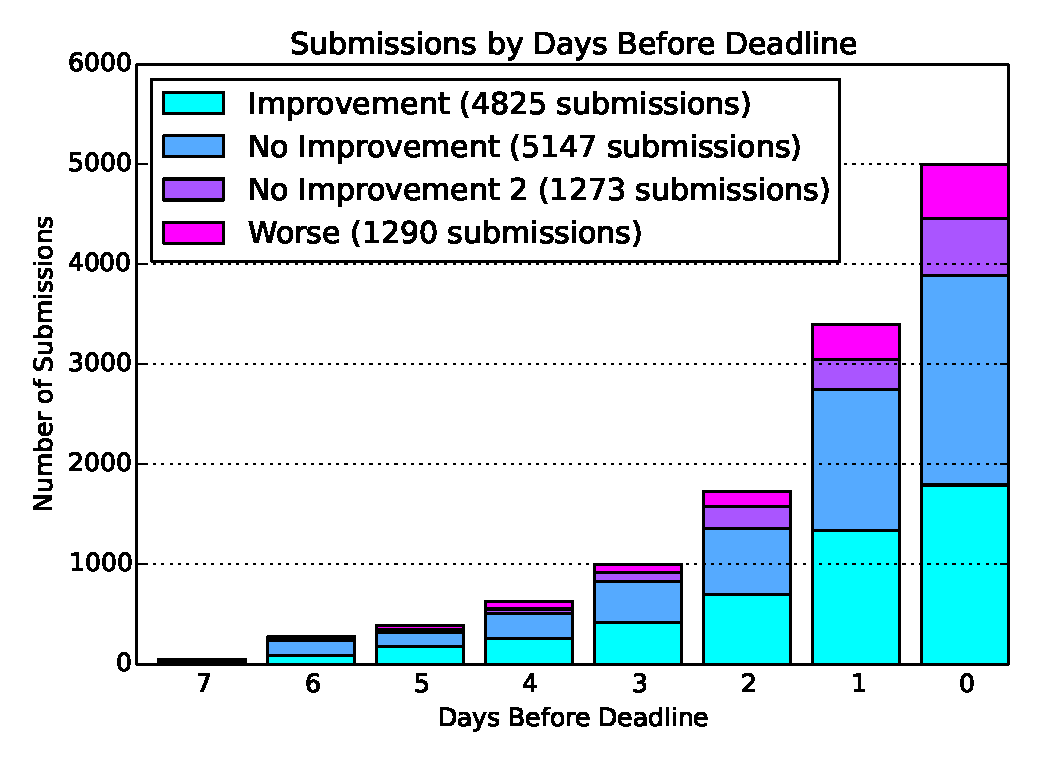
\includegraphics[width=3.3in]{graphs/Submissions_by_Days_Before_Deadline.eps}
\caption{Shows the number of submissions by the number of days each submission
  was made prior to their deadline grouped by improvement category.
  Submissions that improve the group's maximum assignment score are labeled
  \emph{Improvement}, and those that tie are labeled \emph{No
    Improvement}. \emph{Worse} submissions are those that result in a local
  minimum, and all submissions between the group's maximum assignment score and
  the local minimum are labeled \emph{No Improvement 2}.}
\locallabel{fig:days_submissions}
\end{figure}

\begin{figure}[!t]
\centering
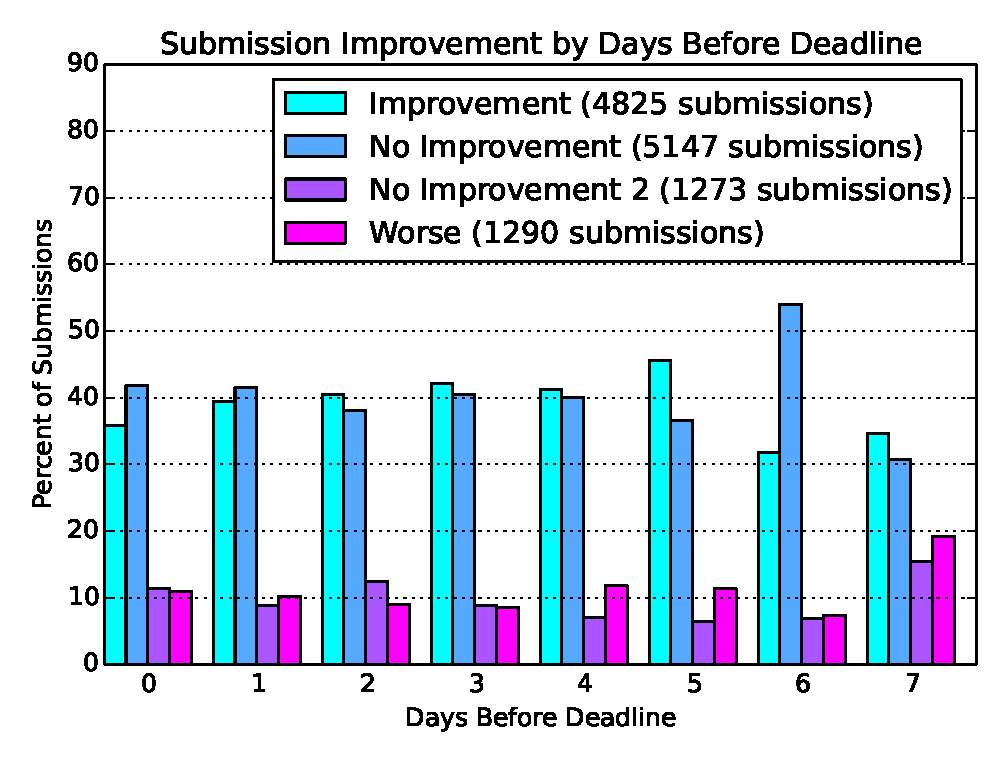
\includegraphics[width=3.3in]{graphs/Submission_Improvement_by_Days_Before_Deadline.eps}
\caption{Depicts the percentage of submissions in each improvement category by
  the number of days each submission was made prior to its deadline.}
\locallabel{fig:days_improvement}
\end{figure}

The previous section describes how submission behavior is altered by assignment
deadlines. In this section we look at the effect of a pending deadline on
submission efficiency. There are a number of ways to define submission
efficiency. One metric is to look at the amount of change in source code
between submissions. Another is to look at the change in cyclomatic complexity
between submissions. While each of these metrics may provide interesting
insights into student behavior, we are more interested in correlations with
changes in groups' scores between submissions. Thus, we consider efficiency by
looking at improvements and regressions in subsequent submissions based on the
change in score between submissions. A change in score is a result of a
subsequent submission passing more or fewer test cases. We quantify changes in
submission efficiency by classifying subsequent submissions into one of four
categories:

\begin{description}
  \item[Improvement] \hfill \\ The submission increases the group's maximum
    score on the assignment.
  \item[No Improvement] \hfill \\ The submission has the same score as the
    group's maximum score.
  \item[No Improvement 2] \hfill \\ The submission's score is less than the
    group's maximum score and is not lower than the local-minimum score.
  \item[Worse] \hfill \\ The submission results in a local-minimum score. That
    is, it is the lowest score since the last \imp{} submission.
\end{description}

Figure~\localref{fig:days_submissions} depicts the total number of submissions
made in the days prior to each submission's respective deadline according to
their respective category. The figure only extends to seven days, as the number
of submissions more than seven days prior to their deadline is
insignificant. Our results show that a majority of submissions are made in the
two days prior to their deadline; this observation is consistent with
\spacco[.]{} In contrast, however, we observe a much higher percentage of
\imp{} submissions when compared to \spacco{}'s \emph{positive}
snapshots~\cite{Spacco:2013:TIP:2462476.2465594}.

The likely reason for this discrepancy is the difference between their
passively collected snapshots and our actively collected submissions. While a
snapshot may not represent a complete unit of work, a submission often does
because groups explicitly make submissions in order to receive feedback. One
other difference is our \imp{} submissions are only submissions that improve
upon a group's maximum score. It is unclear from \spacco{}'s description if a
snapshot that improves the score of a \emph{negative} snapshot is considered
\emph{positive} even if its score does not improve the group's maximum
score. If this is the case, then the number of \emph{positive} snapshots is
inflated in their results as compared to ours.

Regardless, we think a comparison of efficiency between submissions is more
interesting than a comparison between snapshots, because, despite submissions
representing a unit of work, there are still a significant number of
submissions that are not \imp{}. Figure~\localref{fig:days_improvement} shows
the relative percent of submissions in each category by the number of days
prior to their deadline. Overall, the difference in submission efficiency is
insignificant with respect to the number of days prior to assignment
deadline. While our deadlines were distributed such that 24\% and 25\% of
submissions were made to assignments with a Monday and Friday deadline
respectively, there was no difference in submission efficiency with respect to
the day of week a submission was made.

An analysis of the hour of day of each submission also resulted in no
significant changes in submission efficiency. Thus, these results convince us
that time pressure does not affect submission efficiency.

\subsection{Why Do Students Submit Well After an Assignment's Deadline?}
\locallabel{sec:deadline}

\begin{figure}[!t]
\centering
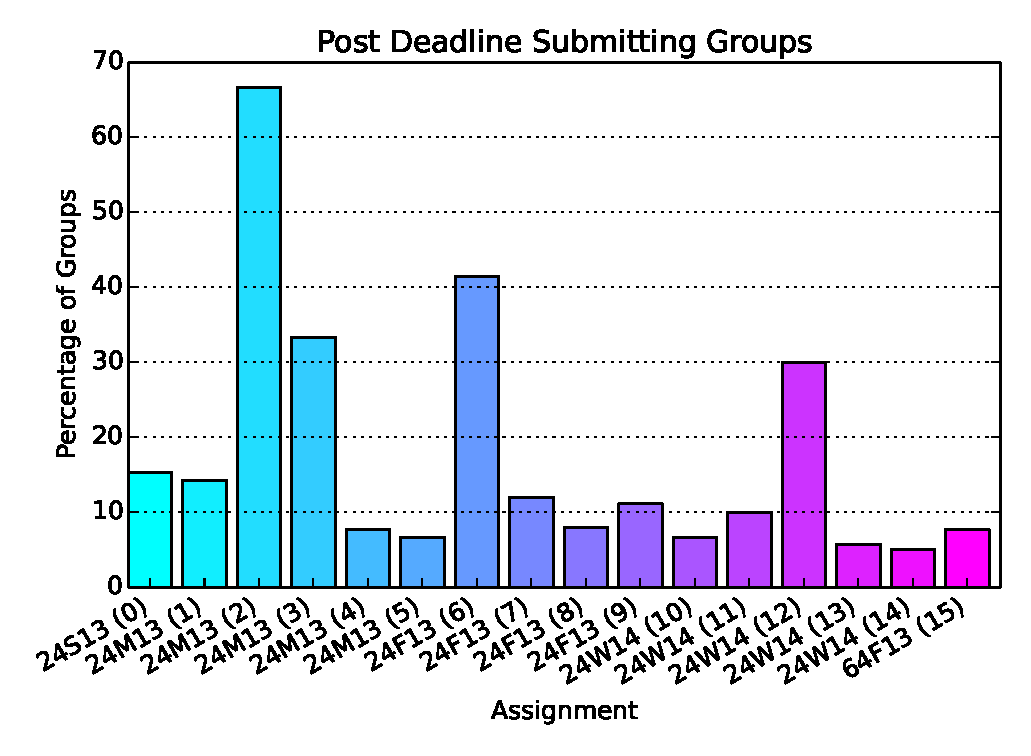
\includegraphics[width=3.3in]{graphs/Post_Deadline_Submitting_Groups.eps}
\caption{Shows the percentage of groups that submit more than two days
  following an assignment's deadline. The x-axis groups the assignments by
  class.}
\locallabel{fig:late}
\end{figure}

An interesting aspect of real-time feedback and assessment systems that prior
work has not touched upon, is student usage of these systems beyond an
assignment's deadline in order to make improvements to their work and verify
the correctness of those improvements. These systems inherently provide this
functionality, and some students take advantage of it.

Figure~\localref{fig:late} shows the percentage of groups by assignment that
made one or more submissions more than two days following an assignment's
deadline. Of the seventy-six assignments, only sixteen are shown in the
figure. Five (6.6\%) assignments were excluded for representing fewer than ten
groups. A majority of these assignments were the first assignment of a class
for which we had only received a portion of the consent forms. Twenty-nine
assignments (38.2\%) had zero post-deadline submitting groups and are therefore
not shown. Finally, twenty-six (34.2\%) assignments had only between 1\% and
4\% (average 2.4\%) of groups with post deadline submissions. These assignments
are excluded from the figure for space purposes.

A minimum of two days following an assignment's deadline was chosen, because by
this time all students were beyond any late-credit that may have been offered
across all assignments. Except where otherwise noted, submissions occurring
after this two-day period provided the student with no direct grade-benefits.

Five of the assignments in Figure~\localref{fig:late} are from \cm[24]{13},
which comprised only seventeen consenting students whereas the next smallest
class, \cs[64]{14}, comprised forty-eight consenting students. \cm[24]{13}'s
small class size is significant as a higher percentage of the students were
able to receive assistance in office hours from both the teaching assistant and
the instructor.

Additionally, five of the assignments are from \cw[24]{14}. In this class, half
of the groups submitting post deadline did so for more than one assignment. We
discovered that the majority of these post deadline submissions occurred just
prior to one of \cw[24]{14}'s course examinations. This discovery suggests that
a number of students utilized the real-time feedback and assessment system as a
tool for exam preparation. Messages on the course discussion group confirmed
students utilized the feedback and assessment system to improve upon previous
course assignments as a form of studying.

Overall, four of the assignments, \emph{2}, \emph{3}, \emph{6}, and \emph{12},
stand out from the remainder. The first two, \emph{2}, and \emph{3}, were
assignments that subsequent assignments depended on. Thus, as reported by the
instructor, many students sought help during office hours to correct issues
with the former assignment prior to moving on to the latter. The instructor
reported that the real-time feedback and assessment system was invaluable
during office hours for its capability to efficiently verify correctness of
modifications to students' code without exposing the test cases, nor requiring
the instructor to manually obtain and test the students' in-progress
work. Assignment \emph{6} presented students with the opportunity to make-up
missed points after the deadline, thus not surprisingly, explaining its spike
in post deadline submissions. Finally, assignment \emph{12} had both a number
of students revisit prior to a class exam, and was a dependency of a subsequent
assignment.

In summary, our results show that there are three primary reasons why students
continue to work on assignments well after the deadline:

\begin{itemize}
\item Intuitively, the most prominent reason we observed is to make up points
  lost on an assignment. While abusing this functionality may result in
  students not taking initial assignment deadlines seriously, the ability for
  instructors to easily reassess student work provides a paradigm of assignment
  assessment that has never before been feasible.
\item The second most prominent reason we observed is due to inter-assignment
  dependency. When an assignment depends on the work of a former assignment, a
  number of students found it useful to first verify correctness of
  improvements made to the former assignment before advancing to the latter.
\item Finally, we observed a small number of students who made improvements to
  past assignments as part of studying for their examinations.
\end{itemize}

Overall we consider any submissions made after the deadline to be a success of
the real-time feedback and assessment system. Without lowering the barriers to
additional feedback, these students may not have made any effort to improve
their comprehension of the material through improvements to their past
assignments.

\subsection{Does Delaying Feedback Impact Student Submission Behavior?}
\locallabel{sec:sub_impact}

\begin{figure}[!t]
\centering
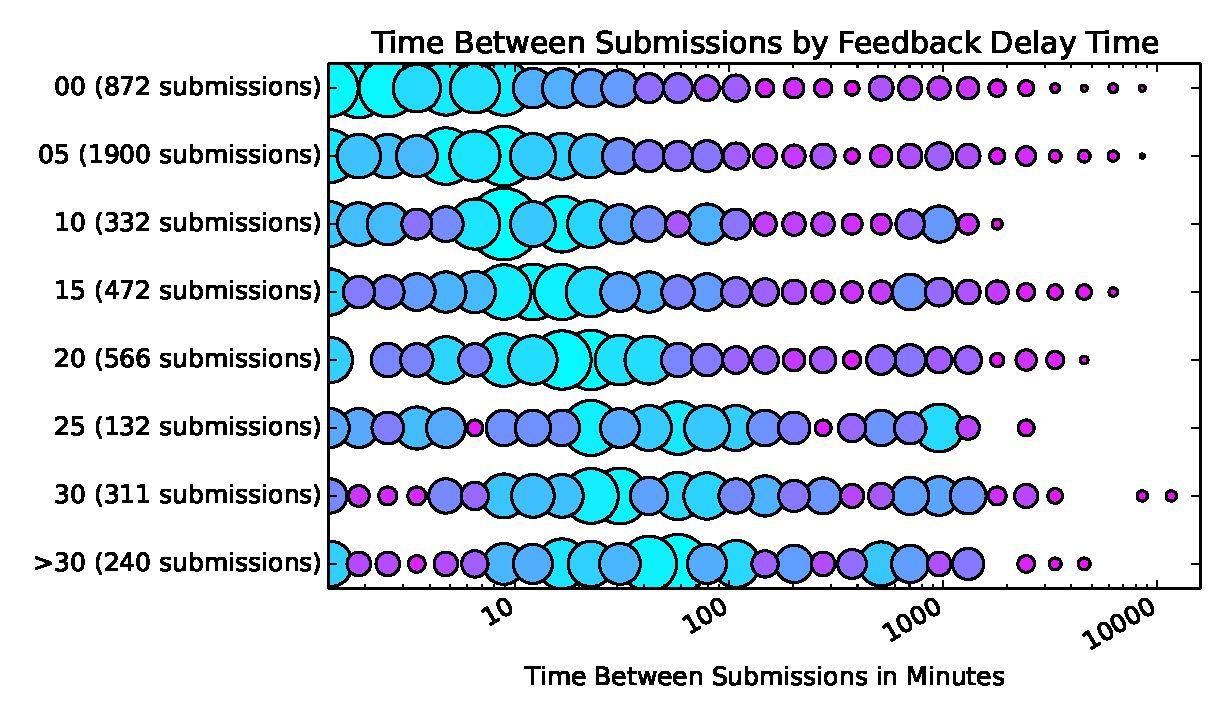
\includegraphics[width=3.3in]{graphs/Time_Between_Submissions_by_Feedback_Delay_Time.eps}
\caption{Plots the time between submissions grouped by assignment feedback
  delay. Note the shift to a longer time between submissions in the most
  significant portion of each row, as indicated by the larger circles, as the
  feedback delay increases.}
\locallabel{fig:delta_delay}
\end{figure}

\begin{figure}[!t]
\centering
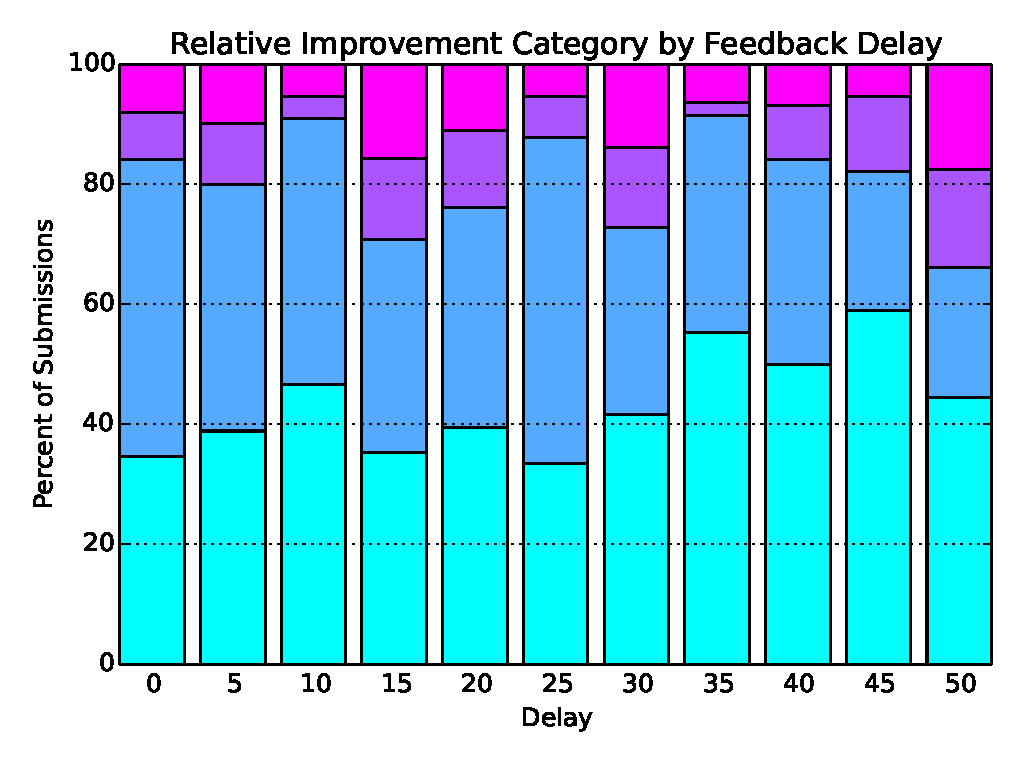
\includegraphics[width=3.3in]{graphs/Relative_Improvement_Category_by_Feedback_Delay.eps}
\caption{Plots the percent of submissions in each improvement category for each
  five-minute delay interval from zero to fifty. Refer to
  Figure~\localref{fig:days_submissions} for the legend and its description.}
\locallabel{fig:delta_efficiency}
\end{figure}

\begin{figure}[!t]
\centering 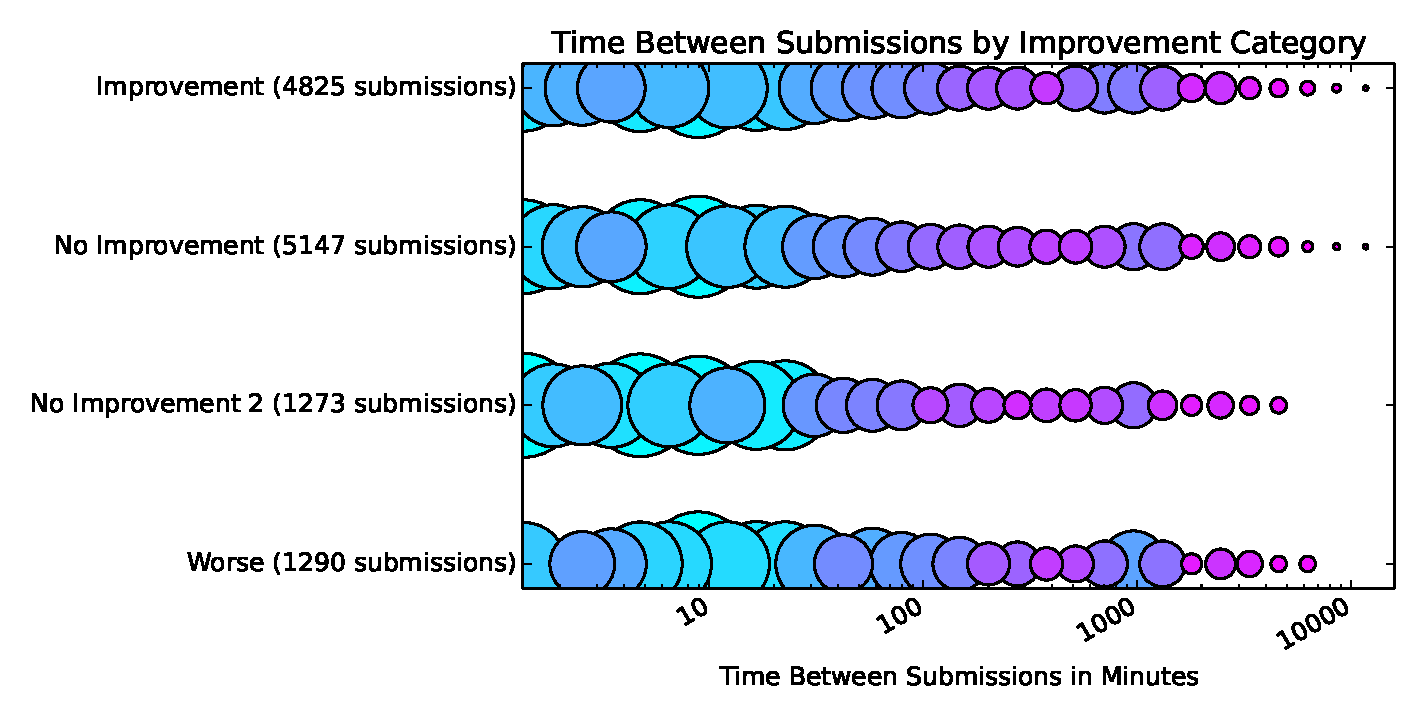
\includegraphics[width=3.3in]{graphs/Time_Between_Submissions_by_Improvement_Category.eps}
\caption{Plots the time between submissions by their improvement category.}
\locallabel{fig:delta_category}
\end{figure}

As indicated in Section~\localref{sec:delay}, we sought to measure the impact
of altering assignment feedback delay on student submission behavior. Here, we
first look at the impact of the feedback delay on the time between subsequent
submissions made by the same group. Figure~\localref{fig:delta_delay} plots the
time between subsequent submissions grouped by assignments sharing the same
feedback delay value to a five-minute precision and combining those with a
feedback delay of more than thirty minutes. Note that the x-axis is shown in a
log-scale, and the size and color of each circle represents the relative number
of submission gaps represented by that circle. For instance, with a feedback
delay of ten minutes, the most significant gap between subsequent submissions
is around ten minutes as indicated by the bright cyan large circle in that
position. This figure clearly shows by the shift in position of the bright cyan
large circles in each row, that as the feedback delay increases, so does the
most significant grouping of subsequent submission gaps. This result indicates
that delays in feedback affect student submission behavior.

Figure~\localref{fig:delta_efficiency} shows the relative efficiency of
submissions grouped by the feedback delay. This figure appears to indicate that
there is a significant improvement in submission efficiency with delays of
thirty minutes or more. Using Student's t-test, we compared the percent of
\imp{} submissions for each feedback delay fewer than thirty minutes, to those
of each feedback delay thirty minutes or longer. The difference was
statistically significant with P=0.0095.

For comparison, Figure~\localref{fig:delta_category} depicts the time between
submissions for each of the improvement categories. The aggregate results from
the figure indicate that the most common time between subsequent submissions is
approximately ten minutes. Furthermore, there is a consistent spike in time
between submissions just prior to the 1,000-minute mark. This time corresponds
with a diurnal working pattern of our students. Overall, there is not a
significant difference in time between submissions with respect to improvement
category. However, the shape of the individual scatter lines provides two
insights:

\begin{itemize}
\item Relatively the most \noii{} submissions occur in the first few seconds as
  indicated by the size and color of the \noii{} category's first circle
  compared with the other categories. Recall that \noii{} submissions occur in
  the period after a \worse{} submission and prior to an \imp{}
  submission. This short period of time between these submissions and their
  corresponding former submissions is too small for a group to have understood
  any feedback received, suggesting these groups did not independently test
  whatever changes they made prior to resubmission.
\item Interestingly, with respect to \worse{} submissions, the spike around the
  1,000-minute mark is the most significant compared to other categories. This
  data suggest that long breaks have an initially negative impact on assignment
  progress.
\end{itemize}

Our results confirm that changes in the feedback delay have an impact on
student submission behavior. In general, as the feedback delay increases
students wait longer to submit, and when comparing delays of less than thirty
minutes to those of thirty minutes or more, the students are more likely to
improve upon their previous score with longer feedback delays.

\subsection{Does Delaying Feedback Impact Student Work Sessions?}
\locallabel{sec:session}

Section~\localref{sec:sub_impact} showed that a delay in feedback has an impact
on both the time between submissions and the likeliness for a group to make an
improving subsequent submission. In this section, we attempt to group
submissions into a work session. Conceptually, a work session is a continuous
period of time that students are actively working on an assignment. Multiple
work sessions are separated by periods of inactivity that may be due to sleep,
distraction, other work, or some other form of break. Grouping multiple
submissions into a work session provides another level of depth to insight on
student behavior. We use these groupings to both look at the effect of the
feedback delay on work sessions, and to compare our work session results to
those of prior work. While our data collection methodology does not allow us to
express work sessions with great precision, we make an approximation.

We define work sessions similarly to \spacco[.]{} Specifically, we define a
work session as a collection of submissions by the same group for the same
assignment in which all subsequent submissions are made within some window of
time to its prior submission. We refer to this window of time as the
\emph{window size}.

\subsubsection{Determining an Appropriate Window Size}
\locallabel{sec:window}

\begin{figure}[!t]
\centering
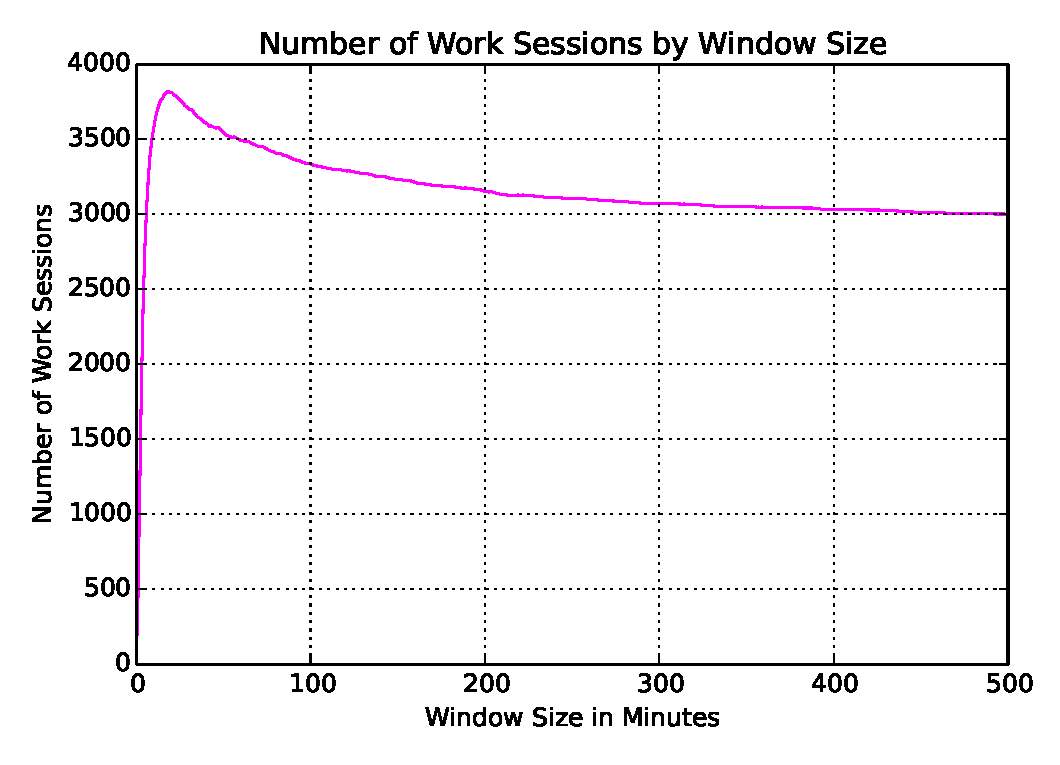
\includegraphics[width=3.3in]{graphs/Number_of_Work_Sessions_by_Window_Size.eps}
\caption{Plots the number of work sessions as the window size increases.}
\locallabel{fig:work_sessions}
\end{figure}

\begin{figure}[!t]
\centering
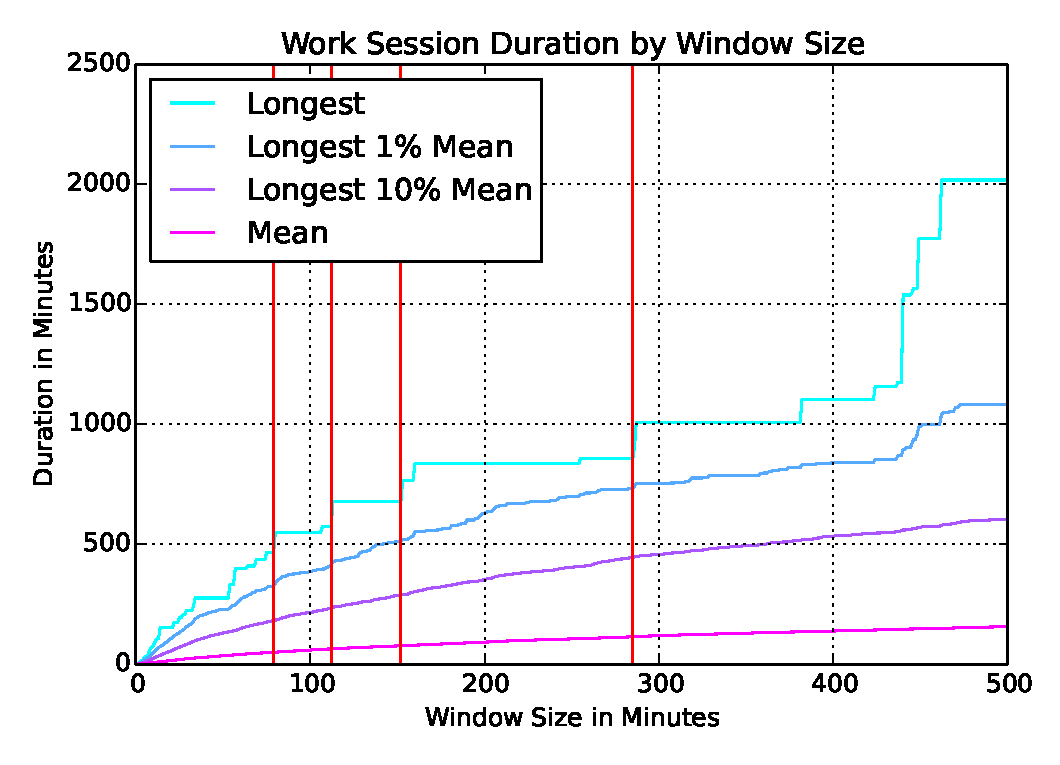
\includegraphics[width=3.3in]{graphs/Work_Session_Duration_by_Window_Size.eps}
\caption{Shows the change in work session duration as the window size
  changes. The red vertical lines indicate points of interest due to
  significant changes in the longest duration work session. The red lines occur
  at window sizes 79, 112, 152, and 285.}
\locallabel{fig:window_size}
\end{figure}

We investigate the ideal window size for which to discover work
sessions. \spacco{} arbitrarily chose a window size of twenty
minutes~\cite{Spacco:2013:TIP:2462476.2465594}. While this window size may have
been appropriate for their data, where snapshots were collected passively upon
changes to students' code, it is not appropriate for our data due to the fact
that students actively submitted only when they desired feedback. Furthermore,
it would not make sense for us to define a window size fewer than fifty minutes
due to inclusion of assignments with a feedback delay of fifty minutes, where
groups regularly make no more than one submission in any fifty-minute
period. Thus, the window size we select must be at least fifty minutes in
length.

There are two forms of error that we must mitigate when selecting a window
size:

\begin{itemize}
\item The first error is due to not being able to distinguish between work and
  non-work time occurring between submissions in a work session. While a
  student may make two submissions in a period of time shorter than the window
  size, they may not have worked for the entire period between those two
  submissions. Intuitively, this error is reduced by minimizing the window size
  due to the fact that any non-work periods longer than the window size will
  not be included as part of the work session.
\item The second error is a result of selecting a window size that is too small
  to encompass actual periods of student working time between two submissions.
  For instance, if we select the window size as sixty minutes, then this error
  corresponds to the number of subsequent submissions representing more than
  sixty minutes of actual work.
\end{itemize}

Although we can measure the number of subsequent submissions over a given
window size, we cannot measure either error due to a lack of information as to
when students are actually working. We accept these errors, and assume that
they equally effect working sessions independent of the feedback delay
time.

Rather than arbitrarily choosing a value, we attempt to select an ideal window
size based on features of our data. We use the maximum session length as a
heuristic for limiting the window size, as it is unlikely that more than a
handful of all sessions are longer than eight hours in addition to time to
account for the error in work time between two
submissions. Figure~\localref{fig:work_sessions} shows the effect of increasing
the window size on the number of work sessions created. This figure reveals
that for our data the maximum number of work sessions occurs with a window size
of approximately twenty minutes, after which the number of work sessions
gradually decreases. This decrease indicates that as the window size grows, the
number of work sessions merged together is more significant than the number of
new work sessions created by the grouping of two independent submissions. Aside
from the twenty-minute peak, there are no other points of interest in this
figure.

Figure~\localref{fig:window_size} plots a number of lines corresponding to
various work session lengths as the window size increases. The four
non-vertical lines correspond to:

\begin{itemize}
\item the duration of the single longest work session
\item the mean duration of the top 1\% of work sessions sorted by length
\item the mean duration of the top 10\% of work sessions sorted by length
\item the mean duration of all work sessions
\end{itemize}

Of these four lines, we find only the duration of the single longest work
session to be of interest as there are a number of distinct window sizes that
result in increasing the longest duration. The red vertical lines on the figure
highlight the window sizes of interest, i.e., they are the window sizes just
prior to a significant increase in maximum work session length. We excluded
consideration of points of interest at larger window sizes due to the
infeasibility for 10\% of all work sessions to be over eight hours in
length. Additionally, we exclude the point of interest that occurs just after
fifty minutes due to its proximity with our longest feedback delay.

We select the left-most point of interest, seventy-nine minutes, as the window
size we use in the remainder of the results section. Note, however, that where
statistical significance is concerned, we verified that each highlighted window
size in Figure~\localref{fig:window_size} produces consistent results with
those produced using the seventy-nine minute window size. This comparison shows
that our analysis is unaffected by the specific choice of window size from the
options we highlighted with red lines.

\subsubsection{Properties of Work Session Lengths}

\begin{figure}[!t]
\centering 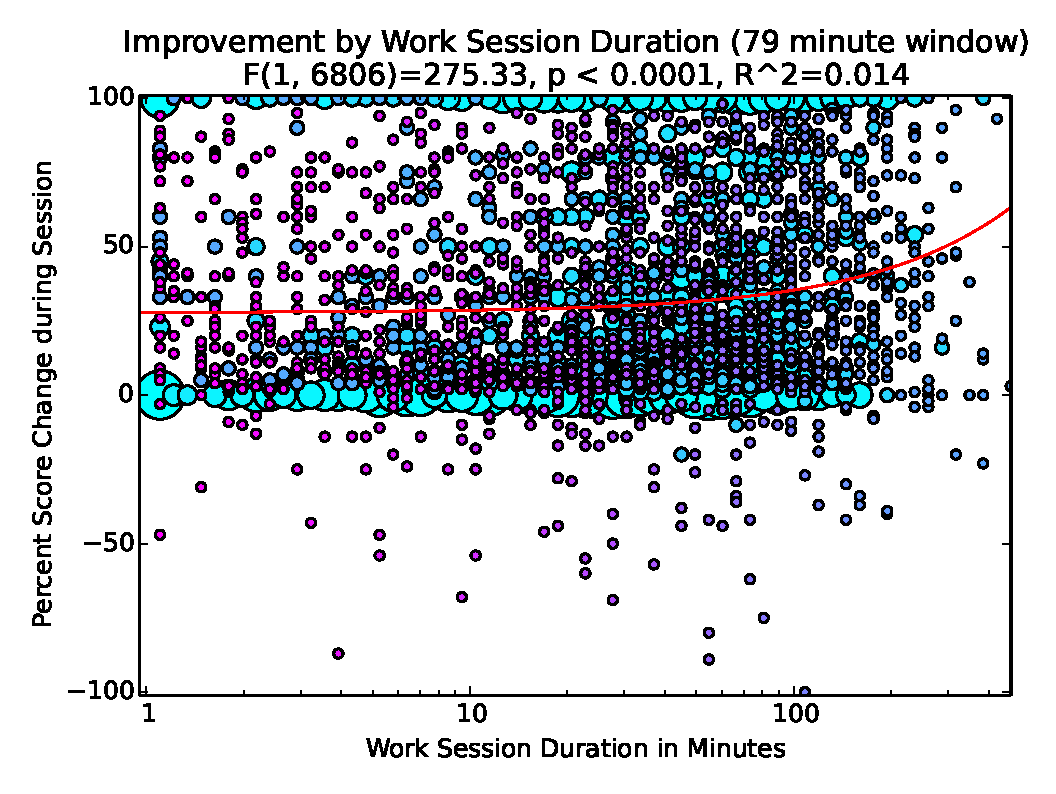
\includegraphics[width=3.3in]{graphs/Improvement_by_Work_Session_Duration_(79_minute_window).eps}
\caption{Depicts a positive correlation between work session duration and
  percent score change. The results are statistically significant according to
  an F-test.}
\locallabel{fig:session_improvement}
\end{figure}

\begin{figure}[!t]
\centering 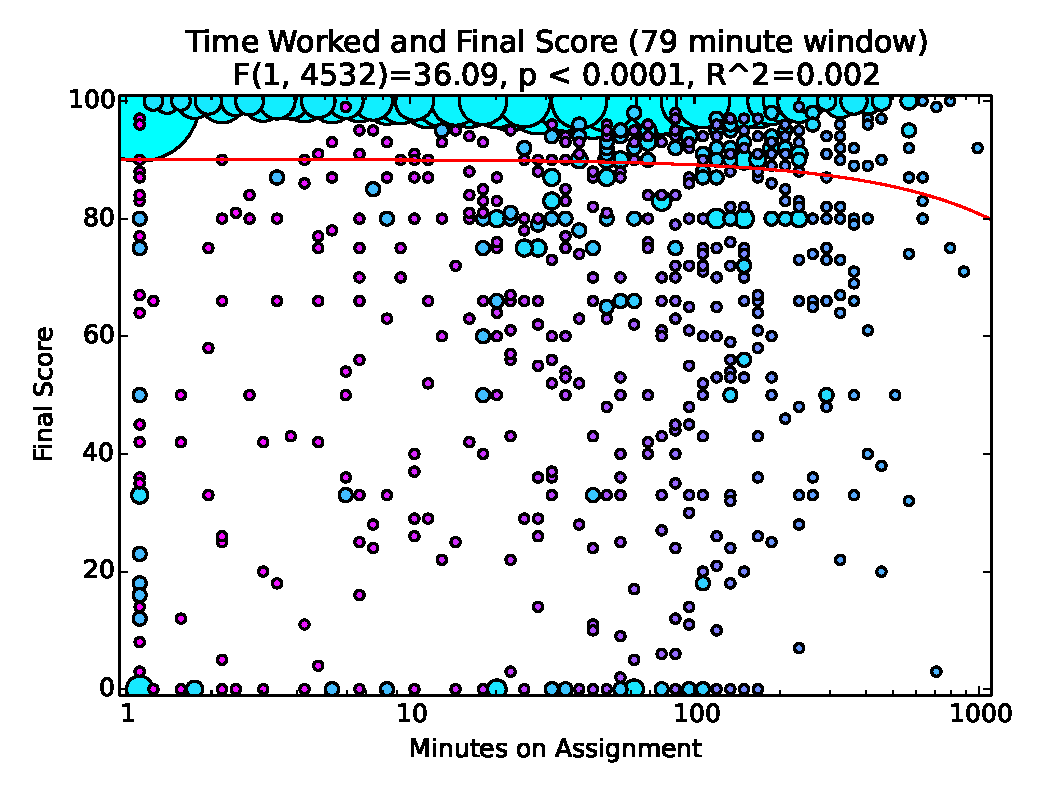
\includegraphics[width=3.3in]{graphs/Time_Worked_and_Final_Score_(79_minute_window).eps}
\caption{Depicts a negative correlation between the minutes spent on an
  assignment and the final score. The results are statistically significant
  according to an F-test.}
\locallabel{fig:time_score}
\end{figure}

\begin{table}
\centering
\begin{tabular}{|c||c|c|c|c|c|} \hline
Score & Count & Mean Work Time & stderr & No Progress & stderr \\ \hline \hline
0\% & 142 & 54m & 6 & 50\% & 4 \\ \hline
0\%--100\% & 616 & 119m & 6 & 58\% & 2 \\ \hline
100\% & 1509 & 60m & 2 & 34\% & 1 \\ \hline
\end{tabular}
\caption{Lists properties of group work times (79 minute window) grouped by
  those that scored 0\%, between 0\% and 100\%, and 100\%. The \emph{mean work
    time} is the mean time groups in each grouping spent working on the
  assignment along with the corresponding \emph{stderr}. \emph{No progress}
  represents the mean percent of time that groups in each grouping spent
  without improving their maximum score.}
\locallabel{table:times}
\end{table}

Before considering the impact of the feedback delay on work sessions, we first
compare a few general properties of our work sessions to the passively
collected work sessions of \spacco[.]{}

Having defined a window size, we are able to group submissions into work
sessions, and thus approximate the length of a work session as the time between
the first and last submission in a work session. Rather than looking at the
improvement between individual submissions as we did in
Figure~\localref{fig:delta_category}, Figure~\localref{fig:session_improvement}
plots the percent score change made between the first and last submission in a
work session against the length of the work session. In this figure circles at
0\% score change on the y-axis would be considered \noi{}, and a vast majority
of changes in work sessions would be considered \imp{} due to the significant
imbalance between the number of sessions that improve the score when compared
to those that reduce the score. The red line represents the trend-line and an
F-test of the data confirms that there is a statistically significant positive
correlation between the length of a work session and the percent change in
score. This analysis indicates that longer work sessions are more likely to
result in increased improvements in score. These results are consistent with
those of \spacco{}~\cite{Spacco:2013:TIP:2462476.2465594}.

We approximate the total time spent on an assignment by summing the length of
all the work sessions by group for an
assignment. Figure~\localref{fig:time_score} plots the final score compared to
the total time spent on an assignment. The red trend-line shows there is a
statistically significant negative correlation between the total work time and
the final score. This negative correlation indicates that the longer a group
works on an assignment the less likely they are to score well. These results
contradict the results of \spacco{} where they found a statistically
significant positive correlation between the two.

This result intuitively makes sense under the assumption that a majority of
groups who do not complete an assignment do not do so due to a lack of
effort. Although groups who complete an assignment are more likely to start
earlier, these groups, on average, spend much less time working on an
assignment. Table~\localref{table:times} confirms this intuition by showing
that the mean work time of groups who receive 100\% on an assignment is nearly
half that of all groups who receive scores between 0\% and 100\%, with little
error. The \emph{No progress} column shows that groups who complete an
assignment spend a larger percentage of their time improving upon their
assignment score, whereas groups, who do not, spend over 50\% of their
assignment time without making forward progress.

That begs the questions, why are groups who complete an assignment likely to
spend less time on it, and why are these groups more efficient? While we cannot
precisely answer these questions, we offer two possible explanations:

\begin{itemize}
\item In general, successful students simply may have a better understanding of
  assignment material, resulting in more productive work sessions, and overall
  reducing the amount of time to completion.
\item Successful students are more likely to start earlier, thus providing them
  with more opportunity to attend office hours. Students who attend office
  hours gain useful insights to an assignment, resulting in more forward
  progress, and overall reduce the time required to complete an assignment.
\end{itemize}

From the opposite perspective of both explanations we can understand why
unsuccessful students may spend more time on an assignment. Without a directed
approach to completing an assignment, these students may figuratively spin
their wheels requiring significant time with little, if any, progress. In such
cases, if these students are not performing their own testing, and waiting for
feedback from the system, delays in feedback may have a negative effect on
student performance.


\subsubsection{Impact of Feedback Delay on Work Sessions}
\locallabel{sec:session_impact}

\begin{figure}[!t]
\centering
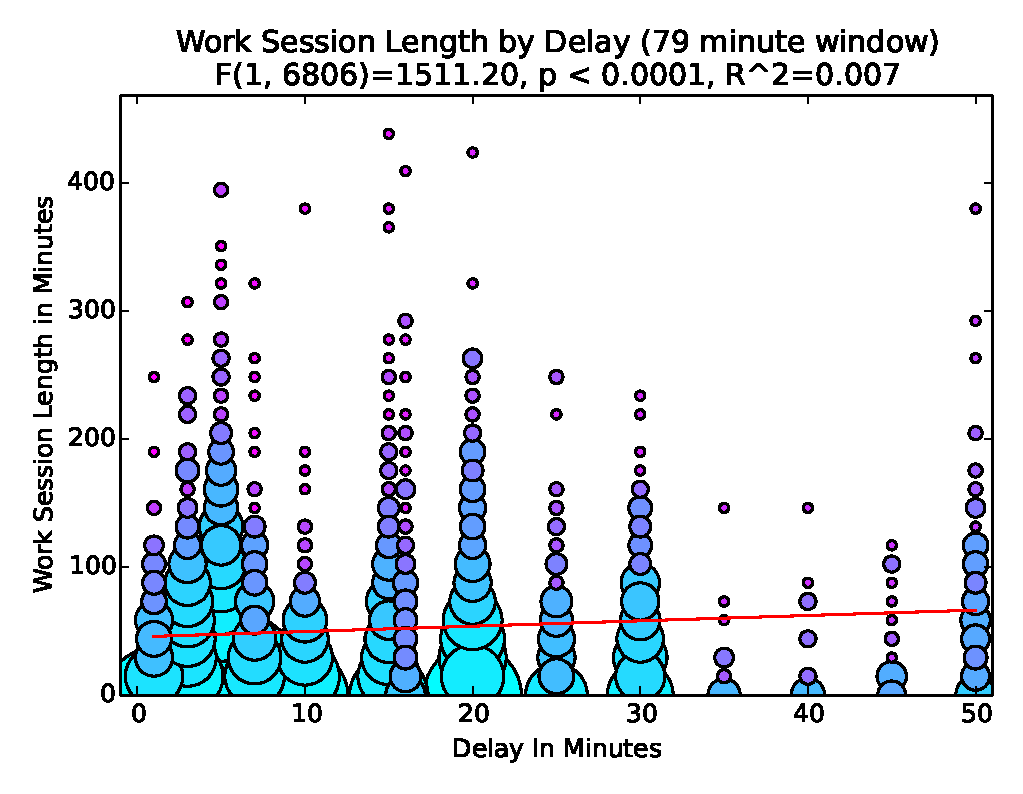
\includegraphics[width=3.3in]{graphs/Work_Session_Length_by_Delay_(79_minute_window).eps}
\caption{Plots work session length against feedback delay. There is a slight,
  nevertheless, statistically significant positive correlation between the
  two.}
\locallabel{fig:session_duration}
\end{figure}

\begin{figure}[!t]
\centering
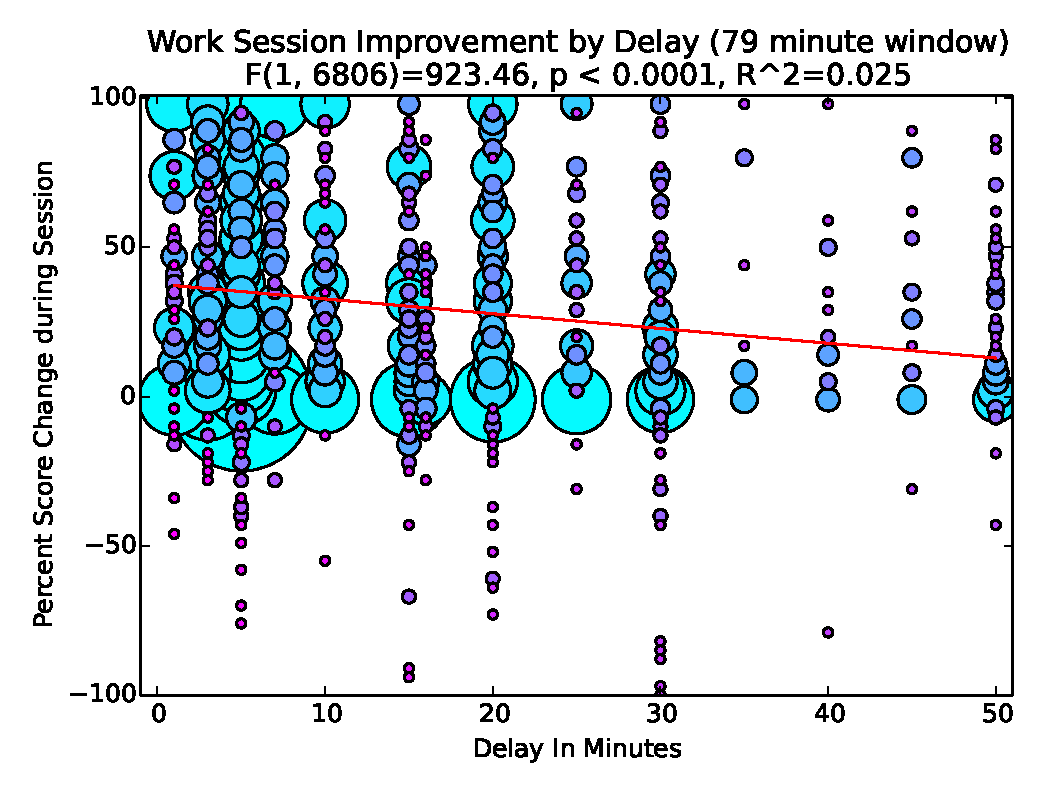
\includegraphics[width=3.3in]{graphs/Work_Session_Improvement_by_Delay_(79_minute_window).eps}
\caption{Plots work session improvement against feedback delay. There is a
  statistically significant negative correlation between the two.}
\locallabel{fig:delay_improvement}
\end{figure}

Finally we consider the impact of the feedback delay on work sessions. We first
consider the effect a change in duration has on the length of a work
session. Figure~\localref{fig:session_duration} shows that there is a
statistically significant, though slight, positive correlation between the
feedback delay and work session length with a seventy-nine minute window
size. The correlation is more prominent with the larger window sizes as
indicated by the red lines in Figure~\localref{fig:window_size}. While we
observe a slight increase in work session length, we cannot absolutely
attribute this to the feedback delay as assignments with delays over thirty
minutes were only given in the latter half of a course. It is common for these
assignments to be more difficult than the initial assignments, and as a result
require more time to complete.

Finally, we look at the impact of the feedback delay on improvement between the
first submission in a work session and the last submission in a work session
when grouped by the feedback delay
value. Figure~\localref{fig:delay_improvement} shows that there is a
statistically significant negative correlation between work session improvement
and the feedback delay. While this result may seem puzzling at first, it is
logical. With a smaller delay, groups have more opportunities to receive
feedback and therefore more significantly improve their work within a single
work session. Thus, while their submission efficiency may be lower, the net
result is increased improvement in the work session. Conversely, with fewer
opportunities for feedback, groups working on assignments with longer delays
have higher submission efficiency but the relative amount of improvement
between work sessions is not as significant.
